\documentclass[tikz, border=2pt]{standalone}
\usepackage{tikz}
\usepackage{amsmath}
\usepackage{xcolor}
\usetikzlibrary{arrows.meta, decorations.pathmorphing, shadings, fadings}
\usetikzlibrary{arrows}
% \usetikzlibrary{pgfmath}
\begin{document}
\begin{tikzpicture}

% =======================================================
% Color definitions (wavelength-labeled)
% =======================================================
\definecolor{c689}{HTML}{FF0000}   % beam 1 (689 nm)
\definecolor{c688}{HTML}{E33434}   % beam 2 (688 nm)
\definecolor{c679}{HTML}{780202}   % beam 3 (679 nm)

% =======================================================
% Layout parameters
% =======================================================

% Beam geometry
\def\rad{4}        % arrow length (beam path radius)
\def\arrspace{1}   % gap between atom cloud and arrow start

% Coordinate-axis inset (bottom-left corner)
\def\ox{-3.7}      % inset origin x
\def\oy{-4.2}      % inset origin y
\def\al{0.8}       % axis arrow length

% Polarization marker size
\def\pollen{0.45}  % half-length of linear polarization arrow

% Gravity marker position
\def\gx{-2.7}
\def\gy{0.4}

% =======================================================
% Styles
% =======================================================
\tikzset{
  beam/.style = {ultra thick, ->, >=stealth, line width=7, font=\Large},
}

% Circle-cross symbol for "into the page" polarization
\newcommand{\polinto}[3]{%
  \draw[#3, line width=1.8pt] (#1,#2) circle (0.28);
  \draw[#3, line width=1.8pt] (#1-0.20,#2-0.20) -- (#1+0.20,#2+0.20);
  \draw[#3, line width=1.8pt] (#1+0.20,#2-0.20) -- (#1-0.20,#2+0.20);
}

% =======================================================
% Beam arrows (three-photon geometry)
% =======================================================

% Beam 3: vertical, from below
\draw[c679, beam]
  (0, -\arrspace-\rad) -- (0, -\arrspace)
  node[midway, left] {$\Omega_3,\; \vec{k}_3$};

% Beam 2: from lower-left at 30 deg
\draw[c688, beam]
  (-150:\arrspace+\rad) -- ++(30:\rad)
  node[midway, above left] {$\Omega_2,\; \vec{k}_2$};

% Beam 1: from lower-right at 150 deg
\draw[c689, beam]
  (-30:\arrspace+\rad) -- ++(150:\rad)
  node[midway, above right] {$\Omega_1,\; \vec{k}_1$};

% =======================================================
% Atom cloud (center of beam intersection)
% =======================================================

% option 1
% \fill[blue!40, opacity=0.15] (0,0) circle (0.8);
% \fill[blue!50, opacity=0.2]  (0,0) circle (0.6);
% \draw[ball color=blue!55!cyan, opacity=0.75] (0,0) circle (0.4);

% option 2
% \shade[inner color=blue!55, outer color=blue!55, opacity=0.08] (0,0) circle (0.85);
% \shade[inner color=blue!60, outer color=blue!40, opacity=0.25] (0,0) circle (0.55);
% \shade[inner color=blue!65, outer color=blue!45, opacity=0.55] (0,0) circle (0.35);


%option 3
% Atom cloud: stippled individual atoms, Gaussian-distributed
\foreach \r/\op in {%
  0.95/0.025, 0.85/0.04, 0.75/0.06, 0.65/0.09,
  0.55/0.12,  0.45/0.15, 0.38/0.18, 0.30/0.20}{
  \fill[blue!55!cyan, opacity=\op] (0,0) circle (\r);
}

% Atoms on top
\begin{scope}
  \pgfmathsetseed{42}
  \foreach \i in {1,...,1000}{
    \pgfmathsetmacro{\x}{0.2*(rnd+rnd+rnd+rnd+rnd+rnd-3)}
    \pgfmathsetmacro{\y}{0.2*(rnd+rnd+rnd+rnd+rnd+rnd-3)}
    \pgfmathsetmacro{\op}{0.3+0.5*rnd}
    \fill[blue!60!black, opacity=\op] (\x,\y) circle (0.015);
  }
\end{scope}

%option 4
% % Atom cloud: layered halos, no specular highlight
% \fill[blue!50!gray, opacity=0.08] (0,0) circle (0.85);
% % \fill[blue!55!gray, opacity=0.12] (0,0) circle (0.65);
% \fill[blue!55!gray, opacity=0.18] (0,0) circle (0.50);
% \fill[blue!60!gray, opacity=0.28] (0,0) circle (0.38);
% \fill[blue!65!gray, opacity=0.45] (0,0) circle (0.25);
% \fill[blue!70!gray, opacity=0.65] (0,0) circle (0.13);

% =======================================================
% Inter-beam angle arcs
% =======================================================
% \draw[black, ultra thick, dash pattern=on 8pt off 4pt, font=\Large, =>stealth]
%   (-148:4) arc (-148:-94:4)
%   node[midway, below ] {$\theta_{23}$};

% \draw[black, ultra thick, dash pattern=on 8pt off 4pt, font=\Large]
%   (-86:4.1) arc (-86:-34:4.1)
%   node[midway, below right] {$\theta_{31}$};

\draw[->,>=stealth',ultra thick, dash pattern=on 8pt off 4pt, font=\Large] (-93:4) arc[radius=4, start angle=-93, end angle=-148]  node[midway, below ] {$\theta_{23}$} ;
\draw[->,>=stealth',ultra thick, dash pattern=on 8pt off 4pt, font=\Large] (-87:4) arc[radius=4, start angle=-87, end angle=-32] node[midway, below right] {$\theta_{31}$} ;


% =======================================================
% Polarization markers
% =======================================================

% Beam 3: linear polarization (double-headed arrow)
\draw[{Stealth[scale=0.7]}-{Stealth[scale=0.7]}, black, line width=1.8pt, font=\large]
  (-\pollen, -\arrspace-\rad-0.15) -- (\pollen, -\arrspace-\rad-0.15)
  node[midway, below] {$\hat{\epsilon}_3$};

% Beam 2: circular polarization (filled dot = into page)
\draw[black, line width=0.1pt, fill=gray!10, font=\large]
  (-150:\arrspace+\rad+0.2) circle (0.1)
  node[above left] {$\hat{\epsilon}_2$};
\draw[black, line width=0.1pt, fill=black]
  (-150:\arrspace+\rad+0.2) circle (0.02);

% Beam 1: circular polarization (filled dot = into page)
\draw[black, line width=0.1pt, fill=gray!10, font=\large]
  (-30:\arrspace+\rad+0.2) circle (0.1)
  node[above right] {$\hat{\epsilon}_1$};
\draw[black, line width=0.1pt, fill=black]
  (-30:\arrspace+\rad+0.2) circle (0.02);

% =======================================================
% Quantization axis (magnetic field direction)
% =======================================================
\draw[-{Stealth[scale=1.4]}, line width=1.6pt, black]
  (1.2, 1.2) -- (-1.2, 1.2)
  node[midway, above, font=\Large, black] {$\vec{B}$};

% =======================================================
% Gravity marker (circle-cross = into page)
% =======================================================
\draw[thick, black] (\gx,\gy) circle (0.22);
\draw[thick, black]
  (\gx-0.16, \gy-0.16) -- (\gx+0.16, \gy+0.16);
\draw[thick, black]
  (\gx+0.16, \gy-0.16) -- (\gx-0.16, \gy+0.16);
\node[right, black, font=\Large] at (\gx+0.25, \gy) {$\vec{g}$};

% =======================================================
% Coordinate-axis inset (bottom-left)
% =======================================================

% Background box
\draw[rounded corners=5pt, gray!30, line width=1.2pt,
      fill=gray!5, draw=gray!40]
  (\ox-1.55*\al, \oy-1.55*\al) rectangle ++(2.2*\al, 2.2*\al);

% x axis (points left)
\draw[-{Stealth}, thick]
  (\ox,\oy) -- ++(-\al, 0) node[left] {$x$};

% y axis (points down)
\draw[-{Stealth}, thick]
  (\ox,\oy) -- ++(0, -\al) node[below] {$y$};

% z axis (out of page — dot-in-circle convention)
\draw[thick] (\ox,\oy) circle (0.18);
\fill         (\ox,\oy) circle (0.05);
\node[above right] at (\ox+0.1, \oy+0.1) {$z$};

% =======================================================
% Inset figure (Doppler-free spectrum)
% =======================================================
\node[anchor=north east, inner sep=6pt] at (7, 4.5) {
  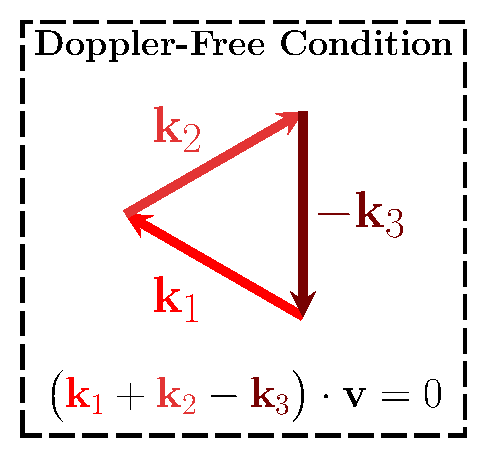
\includegraphics[width=5cm]{doppler_free.pdf}
};

\end{tikzpicture}
\end{document}